\documentclass[twoside, a4paper, openany]{book}

\usepackage[utf8]{inputenc}   % UTF8 character encoding for weird characters
\usepackage[british]{babel}   % Use British english for hyphenation etc
\usepackage{tocbibind}        % Auto add Bibliography etc to Table of Contents
\usepackage[round]{natbib}    % Use BibTeX for bibliography management
\usepackage{hyperref}         % Create hyperlinks within text
\usepackage{geometry}         % Manipulation of page components
\usepackage{marginnote}       % Enable writing in page margins
\usepackage{tikz}             % Inline drawing
\usepackage{multirow}         % Multiple row spanning in tables
\usepackage{tabularx}         % Advanced tables
\usepackage{rotating}         % Full page figures
\usepackage{nameref}          % Enable section reference by name
\usepackage{float}            % Figure positioning

\begin{document}

  \bibliographystyle{plainnat}
% \setlength{\parskip}{0pt}
  % Add a new command \code for inline code formatting
\newcommand{\code}[1]{\texttt{#1}}

  \frontmatter
    \begin{titlepage}
  \newcommand{\HRule}{\rule{\linewidth}{0.5mm}}
  \center

  \textsc{\LARGE Robert Gordon University}\\[1.5cm]
  \textsc{\Large Bachelor of Science in Computer Science}\\[0.5cm]
  \textsc{\large Honours Project Report}\\[0.5cm]

  \HRule \\[0.4cm]
  { \huge \bfseries A platform for Internet-connected Wireless Sensor Networks}\\[0.4cm]
  \HRule \\[1.5cm]

  \begin{minipage}{0.4\textwidth}
  \begin{flushleft} \large
  \emph{Author:}\\
  Stuart \textsc{Whitehead}
  \end{flushleft}
  \end{minipage}
  ~
  \begin{minipage}{0.4\textwidth}
  \begin{flushright} \large
  \emph{Supervisor:} \\
  Dr. Nirmalie \textsc{Wiratunga}
  \end{flushright}
  \end{minipage}\\[4cm]

  {\large 2016}\\[3cm]

  \includegraphics[width=5cm, scale=0.1]{assets/rgu-logo.png}\\[1cm]
  \vfill
\end{titlepage}

    \chapter{Abstract}
  The Internet of Things aims to bridge our physical and digital worlds through innovative technologies, products and services. The purpose of this project is to investigate the current landscape of the Internet of Things, including its main characteristics; why it is attracting attention from large industry players and what challenges have yet to be addressed. The project will pay particular attention to the emerging technologies which are turning this concept into a reality.

  An Internet of Things application framework will be implemented based on the findings from background research. The framework shall support the main capabilities of an IoT system with the aim of being a starting point for other developers and their own applications. A full-stack demonstration application will also be developed using the IoT framework. Not only will this present the opportunity to implement specific IoT technologies, but it will also validate decisions made for the IoT framework.

    \chapter{Acknowledgements}
  I would like to thank everyone who took an interest and showed support for my project---your encouragement has helped me to tackle what has been a challenging but interesting topic.\\

  \noindent In particular I would like thank Dr Nirmalie Wiratunga of Robert Gordon University for her guidance; Marek Pawlowski and Dr Andrew Muir Wood of Mobile User Experience for being the catalysts of my interest in IoT; the guys at FortyTwo Studio for their flexibility and enthusiasm; my parents Alan and May Whitehead for their support and my partner Teri Milton for her encouragement and understanding.

    \input{frontmatter/table-of-contents}
    \input{frontmatter/list-of-figures}
    \input{frontmatter/list-of-tables}

  \mainmatter
    \chapter{Introduction}
  \section{Project Motivation}
  \section{Aims and Objectives}
    % Security as a mindset
  \section{Report Structure}

  \section{Legal, Social, Ethical and Professional Considerations}
  \label{chapter:profession-considerations}
    There are a number of legal, social, ethical and professional issues to consider at all points throughout this project. It is my responsibility and my responsibility alone to ensure that these considerations are upheld.

    The ultimate aim of this project is to satisfy requirements for my Computer Science course---a course which is accredited by the British Computer Society. The BCS maintain a Code of Conduct \citep{bcs-coc} so it is logical that it should inform the responsibilities of this project. More specifically, the code covers four main areas: public interest; professional competence and integrity; duty to relevant authority and duty to the profession.

    \subsection{Public Interest}
      The public interest clause ensures that the legitimate rights of the public and other third parties are respected. With respect to the project focus on the Internet of Things, point 1 (a) of the BCS Code of Coduct should be considered: ``have due regard for public health, privacy, security and wellbeing of others and the environment.''.

      Internet of Things devices have the potential to harvest large volumes of private data about people and places. Health-monitoring devices in particular have the specific capability to measure sensitive medical information; devices like this will not be considered for this project. The devices which have been developed (ambient temperature, colour and gyroscopic motion) are intentionally generic and have no particular privacy requirements. Any users who have been invited to use the devices will be explained as to their purpose.

      The developed application has the capability to store basic identifiable information. In particular, a user profile includes: first and last names; username; password and email address. For the purposes of testing and demonstration, the information database will be seeded with fake data so no user information is at risk. Nonetheless, steps have been taken in order to protect data as far as feasibly possible, including: hardened web hosting with strict a firewall policy; Docker-based deployment environments; random and suitably long alphanumeric passwords for root/admin users.

      Consideration has also been given towards environmental responsibility. Any hardware waste has been disposed of in a responsible manner. For example, spent batteries have been disposed of in a battery bin at a local shop. Hardware devices (wired or battery powered) are switched off when not in use in order to conserve electical power. Documents have only been printed when needed in order to prevent paper wastage. 

    \subsection{Professional Competence and Integrity}
      The professional competence clause ensures that an individual exhibits a true portrayal of their knowledge and capabilities. Effort will be made in every case to understand a topic to the required level. Point 2 (e) is particularly important for the academic nature of this project: ``respect and value alternative viewpoints and, seek, accept and offer honest criticisms of work.''. Opinions and criticisms of this project are welcomed and responses will be made where approriate. 

    \subsection{Duty to Relevant Authority}
      The `Duty to Relevant Authority' clause ensures that due care is exercised with regards to any applicable legislation. First of all, as author I accept responsibility for all work detailed as part of this project. This project will also take all foreseeable measures in order to avoid a conflict of interest with the relevant authority. In the event where information is requested, an approriate response and disclosure will be made.

    \subsection{Duty to the Profession}
      The final clause of the BCS Code of Conduct ensures that the project contributes to and upholds the professional reputation of the computing industry. Point 4 (d) states: ``act with integrity and respect in your professional relationships''. This should be considered with particular attention to software copyright and licensing conditions. Full credit will be given to the authors of software included within the output of this project. Where required, the licensing terms of software (especially Open Source Software) will be upheld.

    \chapter{Background}
  \section{Previous Work}
  \section{Existing Platforms}
  \section{Sensor Hardware}
  \section{Platform Functions}
  \section{Case Studies}
    \chapter{Specification}
\label{Chapter:Specification}
  To obtain a complete and practical understanding of the IoT paradigm, the software implementation accompanying this paper will comprise of two distinct components: a generic IoT application framework and a demonstration application. \citet{interoperability:2015} state that developers of IoT applications would benefit from a generic, standardised architecture, and that is the aim of the framework component. The second component has two main purposes. First of all, it will implemented the framework component with the aim of validating design decisions. The second purpose is to demonstrate the opportunities present in IoT. This chapter will define the requirements for both of these components.

  To help reference these two software components throughout the remainder of this paper, they have been given product names. Haar is a cold sea fog which forms on the east coast of Scotland and is a fitting metaphor for IoT being all around us. It is also a nod towards the Fog Computing paradigm, and towards Robert Gordon University's location in Aberdeen. The generic framework will be called the Haar Engine and the demonstration application will be named Haar.

  \section{Functional Requirements}
    \subsection{Framework}
      The target users of the Haar Engine are designers and developers of IoT services and applications. The general aim of a framework is to encapsulate design decisions into a logical and elegant toolkit. The Haar Engine aims to perform the same task by encapsulating the knowledge which has been collated in Chapter \ref{Chapter:Background}. The following subsection specifies its main requirements.

      \subsubsection{User and Device Management}
        The following requirements have been derived from the analysis of existing platforms and the requirements of use cases.

        \begin{enumerate}
          \item The framework shall model users
          \begin{enumerate}
            \item A user shall be identified by a unique username
            \item A user shall have an associated profile including: full name, email address
            \item Users shall be assigned a privilege level: standard or administrator
          \end{enumerate}
          \item The framework shall authenticate genuine users only

          \item The framework shall model connected IoT devices
          \begin{enumerate}
            \item A device shall be identified by a unique identification number
            \item A device shall be designated as either an input (sensor) or output (actuator)
          \end{enumerate}
          \item The framework shall authenticate genuine devices only

          \item The framework shall authorise and facilitate the management of devices
          \begin{enumerate}
            \item A device will have one owner
            \item Access to device data and configuration options shall be restricted to the device owner by default
            \item The device owner shall be able to make device data public
            \item A device owner shall be able to grant access permission to specified users
          \end{enumerate}
        \end{enumerate}

      \subsubsection{Device Connectivity}
        A main aspect of the IoT concept is the interconnection of devices. The Haar Engine is responsible for managing the connectivity between devices and itself. The issues surrounding bidirectional communication was described in Section \ref{bidirectioncomms}, and these should be addressed by this framework.

        \begin{enumerate}
          \item The framework shall establish a connection with end devices
          \begin{enumerate}
            \item Devices shall be addressable and identifiable whilst the connection is open
            \item The connection shall remain open under normal operating conditions
            \item Under error conditions, the connection shall be re-established
          \end{enumerate}
          \item The connection shall be bidirectional
          \begin{enumerate}
            \item Input devices shall be able to transmit data packets to the framework
            \item The framework shall be able to transmit data packets to output devices
            \item The connection shall be tolerant of network obstacles such as firewalls and Network Address Translation
          \end{enumerate}
        \end{enumerate}

      \subsubsection{Data Storage}
        IoT applications will collect a large volume of data. The data collected by these applications will vary in structure and type, so the Haar Engine must be tolerant of this. The developers potentially using this framework will have specific domain knowledge and so should be empowered to tailor the system for their needs.

        \begin{enumerate}
          \item The framework shall store data received by devices
          \item The framework shall provide an interface for using different database types
          \begin{enumerate}
            \item The framework shall provide a default `out of the box' database connector
            \item Application developers shall be able to create their own database connectors
          \end{enumerate}
        \end{enumerate}

      \subsubsection{Data Access API}
        The Haar Engine must be able to provide access to stored data. Primarily this access will be for use in its own application, however third-party access would enable interoperability between external services and applications.

        \begin{enumerate}
          \item The framework shall provide structured access to stored data
          \begin{enumerate}
            \item Access shall be granted to authenticated and authorised users only
          \end{enumerate}
          \item Application developers shall be able to modify data access
          \begin{enumerate}
            \item Application developers shall be able to add custom data searches
            \item Application developers shall be able to add custom data filters
          \end{enumerate}
        \end{enumerate}

      \subsubsection{Real-Time Event API}
        The ability to react to data in real-time enables novel use cases. As with the Data Access API, the primary purpose is to satisfy the needs of a specific application. However, third-party access to this API would allow for further real-time integrations.

        \begin{enumerate}
          \item The framework shall provide a real-time event API
          \begin{enumerate}
            \item Client applications shall be able to listen for device events
            \item The real-time API shall leverage bidirectional connectivity with devices
          \end{enumerate}
          \item The API shall provide real-time access to data received from devices
          \item The real-time API shall enable developers to create application rules and triggers
        \end{enumerate}

    \subsection{Demonstration Application}
    \label{section:demonstration-application-spec}
      Haar is the second software component for this project. The aim of Haar is to validate the Haar Engine in practice, as well as to demonstrate the opportunities present in the IoT concept. This will be achieved through the implementation of an arbitrary web-based application which sufficiently covers key features.

      \subsubsection{Devices}
        The IoT concept enables the interconnection of devices so this is a logical requirement to begin with. Haar should comprise of at least two separate local device networks to demonstrate global interactivity. These local networks should themselves comprise of a number of devices with enough variety to validate Haar Engine use cases.

        \begin{enumerate}
          \item The application shall comprise of two local area device networks
          \item Devices of these networks shall be capable of establishing a connection between themselves and the web application
          \item The device networks shall comprise of two sensor devices
          \begin{enumerate}
            \item The device network shall contain a sensor device which measures a single data point, such as temperature
            \item The device network shall contain a sensor device which measures more complex data, such as a vector of wind direction and speed 
          \end{enumerate}
          \item The device networks shall comprise of a single actuator device
          \begin{enumerate}
            \item The actuator device shall be flexible enough to represent a variety of data types
          \end{enumerate} 
        \end{enumerate}

      \subsubsection{Dashboard}
        The web-based dashboard will be the main interface between a user and their devices.

        \begin{enumerate}
          \item The dashboard shall be accessible on the World Wide Web
          \item The dashboard shall authenticate users with a username and password
          \item The dashboard shall list profile details
          \item The user shall be able to manage their devices
          \begin{enumerate}
            \item The dashboard shall list devices owned by the user
            \item The user shall be able to add a new device
            \item The dashboard shall show whether devices are connected or not
            \item The user shall be able to transfer ownership of the device
            \item The user shall be able to grant access permissions to other users
          \end{enumerate}
          \item The dashboard shall enable users to manage application rules
          \begin{enumerate}
            \item The dashboard shall list existing rules
            \item The user shall be able to create new rules
            \item An actuator device shall be able to react to sensed data
            \item User devices shall be able to integrate with third-party services
          \end{enumerate}
          \item The dashboard shall display data for a given device [see Data Visualisation below]
          \item The dashboard shall be able to trigger actuators with virtual controls
        \end{enumerate}

      \subsubsection{Data Visualisation}
        There is an opportunity to develop a rich user interface for the dashboard. Since so much of IoT relies on data, it would be appropriate to develop example data visualisation tools for it.

        \begin{enumerate}
          \item A section of the dashboard shall be dedicated to data visualisation
          \item A generic visualisation tool shall plot temporal data as a graph
          \begin{enumerate}
            \item The date range shall be configurable
            \item Multiple data sources shall be comparable on one graph interface
            \item The graph shall leverage the real-time event API to update when new data is received
          \end{enumerate}
          \item Specialised visualisation tools shall reflect specific device types. For example, a virtual thermometer would visualise a temperature
          \begin{enumerate}
            \item Specialised visualisation tools shall leverage the real-time event API to update when new data is received
          \end{enumerate}
        \end{enumerate}

  \section{Non-functional Requirements}
    In addition to the features required for Haar and the Haar Engine, there are a number of additional considerations. Since both of these software components are destined for use in the same system, this section will detail their non-function requirements collectively.

    \subsection{Constraints}
      \subsubsection{Network Environment}
        The potential operating environments in which IoT devices could be implemented vary from domestic household appliances to heavy industrial applications. These networks will all have different configurations, capabilities and customisability. In order to reduce deployment issues, the software components must operate in a common network scenario. A typical home network will be used as a baseline, where only common firewall ports will be allowed.

      \subsubsection{Public IP Address}
        IPv6 is the successor to IPv4 and will allow every connected device to have a unique, globally addressable IP address. While this is the direction the industry is heading in, many businesses and Internet Service Providers are not prepared for its adoption. Network Address Translation (NAT) is still commonly deployed and prevents devices on these networks from being publicly addressable. It should therefore be assumed that end devices will not have a public IP address.

      \subsubsection{Initial Setup}
        In a domestic situation, consumers would be expected to connect products to their internet connection by themselves. This is an important user experience to get right. While this project acknowledges the importance of this, it will not be considered a requirement for Haar so more effort can be afforded to developing a robust application.

      \subsubsection{Sensor Nodes}
        To demonstrate the various framework use cases, the application should connect a variety of sensor types. To ensure this project remains achievable, sensor nodes will be limited to those whose data can be represented by a single data interchange format like XML or JSON. Binary data such as images or audio will not be considered for this project.

    \subsection{Performance Requirements}
      Since this project is a research endeavour, it neither requires nor promises any performance benchmarks. In saying that, the implemented product should meet general performance expectations, especially in regards to any web-based user interfaces.

    \subsection{Security Requirements}
      This particular software product will not store sensitive personal details, nor will it need to satisfy criteria for professional accreditation. However security is an important topic in IoT and so real-world security measures should be implemented. In particular, any device or application connectivity should be implemented over encrypted connections to prevent potential network sniffing. Also any live demonstration versions of this software should be hosted on up-to-date hosting services to prevent any bug exploitations.

    \subsection{Software Quality Attributes}
      \subsubsection{Extensibility}
        The application domain of an IoT project could be in virtually any industry. It is important that this software product is extensible, meaning that the core functionality can be extended to cover specific use-cases.

      \subsubsection{Portability}
        The server infrastructure supporting a generic platform such as this could vary between organisations and use-cases. For instance it may be beneficial to use a Platform as a Service such as Heroku or conversely a range of dedicated servers may be in use. This project should be platform agnostic. 

      \subsubsection{Scalability}
        It is difficult to predict the exact number of sensor nodes and the data which they will produce. The software components should be scalable, either horizontally and/or vertically.

      \subsubsection{Testability}
        It is important that core system functions execute as designed. This project should therefore be testable through assertions where possible and appropriate.

      \subsubsection{Robustness}
        With many devices relying on a system for data and connectivity, system stability is an important focus. The framework should strive to be as fault tolerant as possible, however this is the sum of many parts. Reliable hardware infrastructure and high quality tested code all play a part.

      \subsubsection{Reusability}
        Of course a main feature of a generic framework is the ability to be reused. Two different organisations with different use-cases should both be able to use the framework without issue.

    \chapter{Design}
\label{chapter:design}
   The purpose of this chapter is to document architectural design decisions for Haar and the underlying Haar Engine. It is an important stage in the development of these system components because it combines the requirements specified in Chapter \ref{Chapter:Specification} and the knowledge gained in Chapter \ref{Chapter:Background}. The process has been highly iterative and has led to the upcoming system architecture. 

   One fact which has become clear throughout the design process is that the design and implementation are not mutually exclusive. Some ideas presented in Chapter \ref{Chapter:Background} are dependant on specific technologies, such as the ability to facilitate bidirectional communication (Section \ref{bidirectioncomms}). For this project, the available tools and technologies have therefore informed the design, and this has been integrated to the design process.

   The design process for each functional requirement has consisted of three iterative stages, as shown in Figure \ref{figure:design-process}. First of all, the initial research is consulted to check if any knowledge could inform the design. The requirement and existing knowledge were then used as a basis as a small feasibility investigation for various technologies. Based on these findings, the design was updated. This process was repeated for individual requirements, as well as between requirements to ensure the complete system will operate adequately.

   \begin{figure}
    \centering
      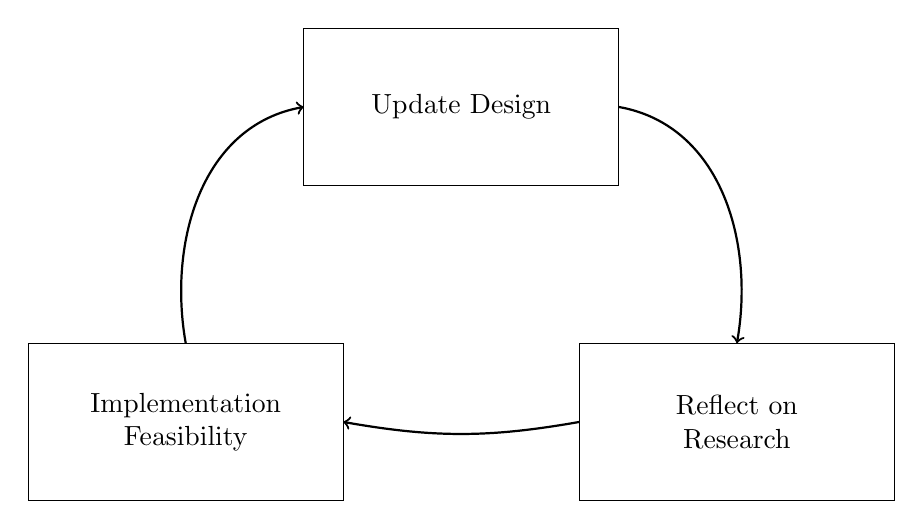
\begin{tikzpicture}
        \node[align=center] at (5.5,5) {Update Design};
        \draw (3.5,4) rectangle (7.5,6);

        \node[align=center] at (2,1) {Implementation\\Feasibility};
        \draw (0,0) rectangle (4,2);

        \node[align=center] at (9,1) {Reflect on\\Research};
        \draw (7,0) rectangle (11,2);

        \path (2,2) edge [->,thick,out=100,in=190]  (3.5,5);
        \path (7.5,5) edge [->,thick,out=350,in=80]  (9,2);
        \path (7,1) edge [->,thick,out=190,in=350]  (4,1);
      \end{tikzpicture}
    \caption{Iterative steps when designing for functional requirements}\label{figure:design-process}
  \end{figure}

  \section{Haar Engine}
    The first component to get design attention is Haar Engine. Since this will support the main system functions required for IoT applications, its design is heavily informed by the available technologies.

    One major design decision is the programming environment used to implement Haar Engine. It is important because it informs how the code can be structured. First of all, the chosen programming language and ecosystem must be able to support the requirements outlined in the previous chapter. Beyond that, the language and framework must provide suitable constructs so application developers can easily extend and modify for their own needs. Various languages and architectures were investigated (such as PHP, Ruby, Python and Go), however one stood out as being most suitable for this project: Node.js.

    Node.js is a server-side implementation of JavaScript. More specifically it implements Google's V8 JavaScript engine and it is ideal for this project due to its event-driven nature. In general, it is based on the event loop concurrency model - a single-threaded process which loops continuously over a message queue \citep{event-loop}. Haar Engine is expected to be focussed on input and output operations. I/O operations using more traditional technologies such as PHP, Python and Ruby are synchronous in nature and block further execution of the process. In comparison, JavaScript can continue processing other instructions while waiting for an IO operation to complete.

    There are various web application frameworks developed on top of Node.js, with the \textit{de facto} standard being Express. The Express framework is based on the concept of middleware, where middleware functions anonymously pass objects to the next one until a web request has been completed. This concept could therefore be used to an advantage for system aspects like authentication.

    Bearing these language features in mind, a final design for the framework has been defined. A logical view of the main system components can be seen in Figure \ref{figure:framework-architecture}. The design decisions for each of these framework components have been described in the following subsections.

    \begin{figure}
    \centering
      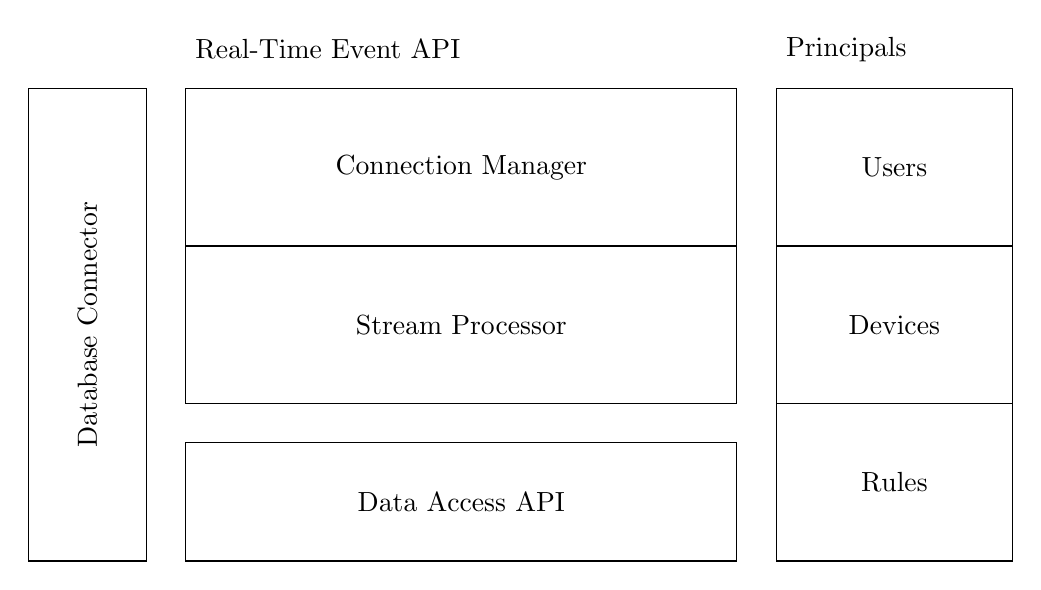
\begin{tikzpicture}
        \draw (0,0) rectangle (1.5,6);
        \node[align=center, rotate=90] at (0.75,3) {Database Connector};

        \draw (2,2) rectangle (9,6);
        \draw (2,4) -- (9,4);
        \node[anchor=west] at (2,6.5) {Real-Time Event API};
        \node[align=center] at (5.5,5) {Connection Manager};
        \node[align=center] at (5.5,3) {Stream Processor};

        \draw (2,0) rectangle (9,1.5);
        \node[align=center] at (5.5,0.75) {Data Access API};

        \draw (9.5,0) rectangle (12.5,6);
        \draw (9.5,4) -- (12.5,4);
        \draw (9.5,2) -- (12.5,2);
        \node[anchor=west] at (9.5,6.5) {Principals};
        \node[align=center] at (11,5) {Users};
        \node[align=center] at (11,3) {Devices};
        \node[align=center] at (11,1) {Rules};
      \end{tikzpicture}
    \caption{A logical view of system architecture for the Haar Engine}\label{figure:framework-architecture}
  \end{figure}

    \subsection{Data Modelling}
      The functional requirements in Chapter \ref{Chapter:Specification} make reference to a number of modellable objects. These are users, devices and rules, and they all have a notion of ownership and authorisation within the framework. During initial research, it was found that an existing platform (Nitrogen.io) abstracts similar objects into a collection called principals. Throughout the design process, users, devices and rules have have proven to be first-class citizens of the framework, so Haar Engine will adopt the same terminology.

      The three principal objects set foundations for the complete data model as well as other framework components, so it is important that they are modelled correctly. This subsection will first describe the traits of each principle before expanding their relationships into an entity-relationship model. Figure \ref{figure:principal-models} illustrates the relationship between the principals.

      \subsubsection{Users}
        The user principal is fundamentally responsible for authorisation within Haar Engine. This will model an end-user account such as an individual person or a company, who will access their account using a unique username and a password. The user is responsible for managing their own devices and rules. Haar Engine will identify user principals with a unique identifier. This would allow users to change their username while maintaining relationships with other principals.

        User principals will be the gatekeeper to devices associated with their account. First of all, they will be able to attach new devices to their account. Users will also have the ability to share access to sensor devices with specific users, or make that data publicly available. Finally, user principals will have the ability to transfer ownership of the device to another Haar Engine user account and relinquish administration control over it.

        User principals will also be able to create, modify and delete rules. When a new rule is created, the user will be designated as the owner of it. Unlike devices, users cannot share rules with another user, nor can they transfer ownership. It is foreseeable that a rule is configured to watch sensor data which is owner by another user. Since access to a third-party sensor cannot be granted, the rule would not have appropriate access permissions to run.

      \subsubsection{Devices}
        The device principal will model a single IoT device. The device can be one of two types (either a sensor or an actuator). Devices will be owned by one user, however further users may be granted access to sensor data. Devices will be identifiable with a unique identifier in Haar Engine. This identifier will be used for the purpose of authentication and authorisation against user principals.

        The device model will also describe the type of data which it supports. For sensor devices, the principal will note the type of measurement (a single value or a vector of values) and the unit(s) of measurement. In the case of actuators, the principal will describe possible output types (single value or a vector of values), as well as value limits. These data type descriptions will be used when defining rules.

      \subsubsection{Rules}
        Rule principals define triggers within the Haar Engine. They are created and owned by a user principal. A rule will consist of a watch target, trigger criteria (such as threshold values), an action target and an action. The watch target is a sensor to monitor and when changes are detected, its output values will be compared against trigger criteria. If the criteria is met, the action target (actuator) will be updated in accordance with the action to take.

      \subsubsection{Entity Relationship Model}
        1. Entity Relationship Diagram using Bachman Notation.

        \begin{figure}[H]
        \centering
          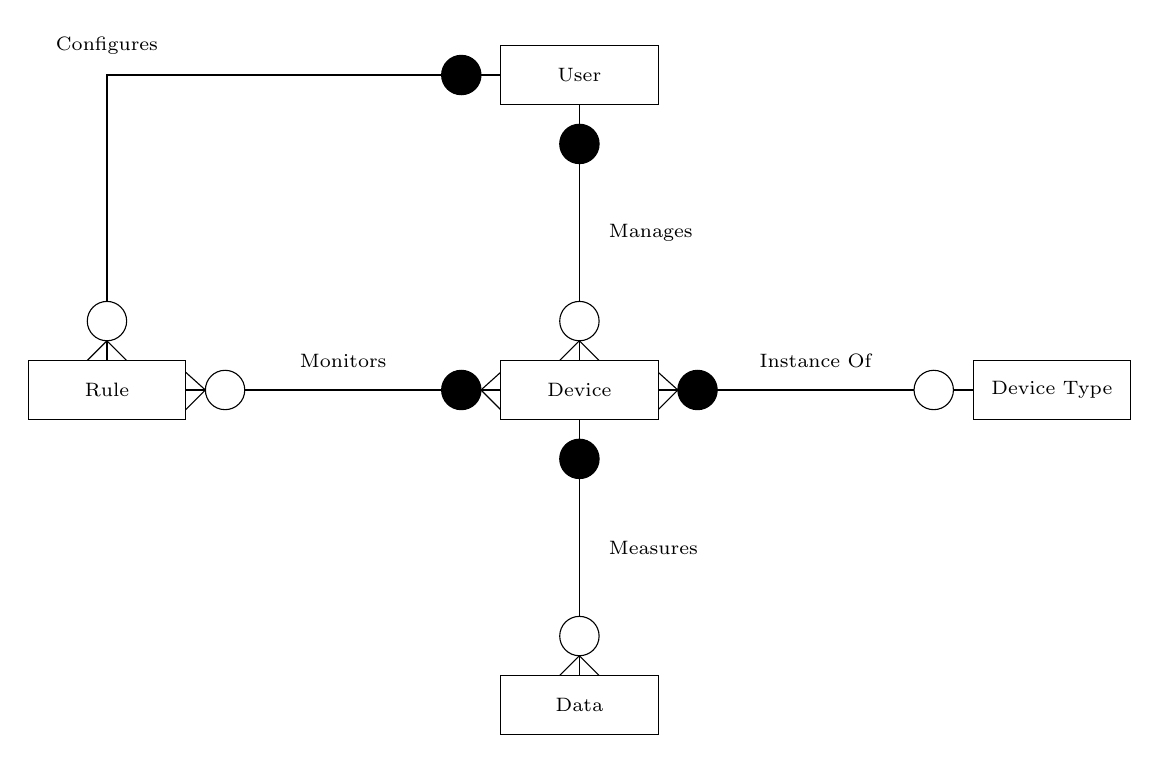
\begin{tikzpicture}
            \tikzstyle{every node}=[font=\scriptsize]

            \draw (7,8) -- (7,0.75);
            \draw (2,4.375) -- (12,4.375);
            \draw (1,4.75) -- (1,8.375) -- (6,8.375);

            \draw[fill=white] (2.5,4.375) circle [radius=0.25];
            \draw (2,4.6) -- (2.25, 4.375) -- (2,4.125);
            \node at (4,4.75) {Monitors};
            \draw (6,4.6) -- (5.75, 4.375) -- (6,4.125);
            \draw[fill=black] (5.5,4.375) circle [radius=0.25];

            \draw[fill=black] (8.5,4.375) circle [radius=0.25];
            \draw (8,4.6) -- (8.25, 4.375) -- (8,4.125);
            \node at (10,4.75) {Instance Of};
            \draw[fill=white] (11.5,4.375) circle [radius=0.25];

            \draw[fill=white] (7,5.25) circle [radius=0.25];
            \node[anchor=west] at (7.25,6.375) {Manages};
            \draw (6.75,4.75) -- (7, 5) -- (7.25,4.75);
            \draw[fill=black] (7,7.5) circle [radius=0.25];

            \draw[fill=black] (7,3.5) circle [radius=0.25];
            \node[anchor=west] at (7.25,2.375) {Measures};
            \draw (6.75,0.75) -- (7, 1) -- (7.25,0.75);
            \draw[fill=white] (7,1.25) circle [radius=0.25];

            \draw[fill=black] (5.5,8.375) circle [radius=0.25];
            \node at (1,8.75) {Configures};
            \draw (0.75,4.75) -- (1, 5) -- (1.25,4.75);
            \draw[fill=white] (1,5.25) circle [radius=0.25];

            \draw (0,4) rectangle (2,4.75);
            \node at (1,4.375) {Rule};

            \draw (6,0) rectangle (8,0.75);
            \node at (7,0.375) {Data};

            \draw (12,4) rectangle (14,4.75);
            \node at (13,4.375) {Device Type};

            \draw[fill=white] (6,4) rectangle (8,4.75);
            \node at (7,4.375) {Device};

            \draw (6,8) rectangle (8,8.75);
            \node at (7,8.375) {User};

          \end{tikzpicture}
        \caption{Entity Relationship Diagram for the Haar Engine}\label{figure:principal-models}
      \end{figure}

      2. Entity Sets
      \begin{itemize}
        \item User(\underline{id}, username, password, role)
        \item Device(\underline{id})
        \item Device Type(\underline{id}, type, structure)
        \item Data(\underline{id}, values)
        \item Rule(\underline{id}, watch target, criteria, action target, action)
      \end{itemize}

      3. Relationships
      \begin{itemize}
        \item Manages --- User manages Device [1:m][m:o]
        \item Configures --- User configures Rule [1:m][m:o]
        \item Instance Of --- Device instance of Device Type [m:1][o:m]
        \item Measures --- Device measures Data [1:m][m:o]
        \item Monitors --- Rule monitors Device [m:1][o:m]
      \end{itemize}

      4. Constraints and Assumptions
      \begin{itemize}
        \item Device Type structure is an array of objects. Each object describes a possible measurement.
        \item The Device Type of a device will never change
      \end{itemize}
    \subsection{Database Connector}
    \label{section:database-connector}
      Efficient data storage is an important performance consideration. The requirements in Chapter \ref{Chapter:Specification} also state that application developers should have the ability to change the database type to suit their own application. The design solution arrived at for this requirement is a database connector API.

      The database connector API will provide a set of foundation methods for operating on principal models and data generated by devices. The framework will use a consistent programming interface and this will allow application developers to change the connector for one of their own design. In a more strictly-typed programming language, object-oriented constructs such as abstract classes or interfaces might be used to define class signatures. With JavaScript, programming techniques like function composition might be more appropriate. 

      Whilst Haar Engine will provide the capability of changing the database connector, an `out of the box' connector will be provided. A NoSQL database fits the purpose of the framework better than an SQL-based database because the data stored could be of varying formats and structures. There are a variety of NoSQL databases available, which will be discussed in the implementation chapter.

    \subsection{Data Access API}
      There are a number of mature standards used for structured data access on the web, so this requirement of the project is about choosing the most appropriate. Two widely-used access standards are Simple Object Access Protocol (SOAP) and Representational State Transfer (REST). These standards also use data interchange formats such as eXtensible Mark-up Language (XML) or JavaScript Object Notation (JSON).

      A REST API was found to be a better fit than SOAP for the Haar Engine. The REST access operators integrate much easier with potential implementation technologies like Node.js and Express and it is a simpler standard to use. The JSON data interchange format is based on JavaScript object constructs so it naturally integrates with a JavaScript-based application.

      Authentication will have to be enforced by every component of the Haar Engine, including the Data Access API. One characteristic of REST APIs is that they are stateless, meaning no session data is stored server-side and that every request will have to be inspected for appropriate access permissions. Two authentication techniques which will be used are a username and password combination, as well as token-based authentication. Clients will first authenticate with their username and password and if accepted, the REST API will return a unique access token for use in subsequent requests.

    \subsection{Real-Time Event API}
      One main characteristic of IoT is the ability to react on sensor data in real-time. This makes a robust and effective real-time API a priority for any given application. Giving structured access to this feature is challenging due to the points described in Section \ref{bidirectioncomms}. For this reason, the problem has been divided into two constituent components: opening and maintaining a true bidirectional communication channel, and efficiently handling messages between the two nodes of the channel.

      One technology which goes some distance in helping with this is MQTT. As described in Section \ref{section:mqtt}, MQTT is a publish-subscribe protocol which facilitates the transmission of messages. MQTT is a very robust protocol however given project constraints and the additional complexity which it might create, it has been deemed unfeasible for this project. Instead, the JavaScript project Socket.io can open and maintain WebSocket connections, with fallbacks if the WebSocket protocol is unavailable. The message-passing concepts of MQTT could be applied to Socket.io.

      \subsubsection{Connection Manager}
        The connection manager is responsible for navigating potential network issues to maintain a bidirectional communication channel. Choosing to use Socket.io and the WebSocket protocol should alleviate any of the issues regarding firewalls and NAT. Socket.io provides an API for managing WebSocket connections. Clients can connect to namespaced URIs which encapsulate different categories of client---Haar Engine will use two default namespaces: sensors and actuators.

        It is also the responsibility of the connection manager to authenticate clients, whether they are users or devices. Socket.io also solves this problem with the use of its own middleware capability. This middleware could make use of authentication mechanisms already in place for the Data Access API.

      \subsubsection{Stream Processor}
        Once a connection has been established, it is the responsibility of the stream processor to act on messages. The Socket.io API allows clients to join one or more rooms within a given namespace and this capability will be leveraged by the stream processor. For example, multiple sensors will each have their own room under the sensor namespace. The stream processor can listen for any sensor events and store the data. Alternatively, stream processing rules (based on the rule principal object) could listen for messages in a single sensor room and act accordingly.

  \section{Haar}
    The main purpose of the second component, Haar, is to validate the implementation of Haar Engine. Most of the heavy lifting will be done by Haar Engine, however this application also requires design attention, especially in regards to the end devices. There are three main components to be investigated: the back-end application, front-end application (dashboard) and the Wireless Sensor Network itself.

    \subsection{Back-End Application}
      The back-end application is simply an instance of the Haar Engine. It is expected that the data models will be extended for one or two application-specific fields (such as a profile picture and biography for users) however it will generally be left as designed. The back-end application will be self-contained and separate from the front-end application. 

    \subsection{Front-End Application}
    \label{section:front-end-application}
      The front-end application is, in essence, simply a user interface for the back-end APIs. It will make use of the Data Access API and Real-Time Event API to manage users, devices, rules and the authentication for all of them. The main challenge presented by the dashboard is handling very dynamic, real-time data in a structured and efficient way for a variety web browsers. The implementation details of this will be discussed in detail as part of the next chapter.

      What can be discussed at this stage is the design, layout and behaviour of the user interface. Figure \ref{figure:desktop-layout} illustrates the general layout which will be used. On desktop-sized web browsers, the window will be split into two panes---one used for navigation, and one for displaying the current page content. On mobile-sized web browsers, only one pane will be displayed at a time. By default, this will be the content pane and when the navigation button is clicked, the navigation pane will be shown.

      The behaviour of the user interface is a challenging aspect. It is expected that aspects of the user interface will react in real-time to new data, so it will also have to open a connection to the Real-Time Event API. This will be possible by using the Socket.io library client-side. The challenges begin when the user starts to navigate to different pages of the dashboard. Traditionally this would load a completely new page, however real-time connections would have to be renegotiated and this is inefficient. Instead, dashboard pages will be loaded asynchronously. Care must then be taken to achieving this in a structured way with in its implementation.

      \begin{figure}
        \centering
          \begin{tikzpicture}
            \node[inner sep=0pt] at (0,0)
              {\includegraphics[width=\textwidth]{assets/desktop-layout.png}};
          \end{tikzpicture}
        \caption{UI layout for desktop-sized web browsers}\label{figure:desktop-layout}
      \end{figure}

    \subsection{Wireless Sensor Networks}
      The third and final component for the Haar application is the Wireless Sensor Network. The WSN comprises of the physical sensors and actuators which create an interface between the physical and digital worlds. To fully demonstrate the capability of the Haar Engine, there is a requirement for a variety of sensor types.

      Before designing individual devices it is first important to plan the data flow between them. It has already been decided that the Haar Engine will support bidirectional communication through the use of the WebSocket protocol, meaning that end devices must also support it. However, to maintain a persistent WebSocket connection any given end device must be awake 100\% of the time. IoT devices should be as power efficient as possible and maintaining a WebSocket connection would prevent them from being able to sleep. Similarly, the WebSocket protocol requires extra software overhead to manage connections; simpler, more efficient protocols already exist for IoT device communication.

      As described in Section \ref{section:connectivity}, ZigBee is a lightweight wireless communication protocol ideal for use in IoT solutions. ZigBee, however, is not compatible with the TCP/IP protocol used for Internet communications. To compromise on this issue, a bridge solution will be used. A bridge device will maintain the WebSocket connection with the Real-Time Event API; when a WebSocket packet is received, the bridge will translate it into a ZigBee packet and vice-versa. This system architecture is shown in Figure \ref{figure:wsn-architecture}.

      \begin{figure}
        \centering
        \begin{tikzpicture}

          \draw (0,1.125) rectangle (2.5, 2.375) node[midway] {Haar API};
          \draw[<->, >=stealth] (2.5,1.75) -- (3.75,1.75);

          \node[cloud, cloud puffs=11, cloud ignores aspect, minimum width=2.5cm, minimum height=1.5cm, align=center, draw] (cloud) at (5,1.75) {Internet};
          \draw[<->, >=stealth] (6.25,1.75) -- (7.5,1.75);

          \node at (7.5, 4.3) {WSN};
          \draw [dashed] (7,-0.5) rectangle (14, 4);

          \draw (7.5,1.125) rectangle (10, 2.375) node[midway] {Bridge};

          \draw (11,2.25) rectangle (13.5, 3.5) node[midway] {Sensor};
          \draw[<-, >=stealth] (10,2.0625) -- (10.5,2.0625) -- (10.5,2.875) -- (11,2.875);

          \draw (11,0) rectangle (13.5, 1.25) node[midway] {Actuator};
          \draw[->, >=stealth] (10,1.4375) -- (10.5,1.4375) -- (10.5,0.625) -- (11,0.625);
        \end{tikzpicture}
      \caption{System architecture for Haar devices}\label{figure:wsn-architecture}
    \end{figure}

      \subsubsection{End Devices}
        To successfully demonstrate the IoT framework, a number of devices are required. Ideally, these devices should be a true representation of an IoT device and not just mocked using software emulation. For the purpose of this project, a true IoT device is considered as having constrained resources, low power and inexpensive components.

        Out of the hardware platforms investigated in Section \ref{sensor-hardware}, the Arduino development platform is the most suited. The Arduino hardware boards and software tools are open source giving complete transparency to their implementation. The Arduino IDE also comes packaged with all the software required to develop and compile the c/c++ based programs. There are a variety of hardware boards and accessories and they are all inexpensive and widely available.

        Most Arduino boards have limited connectivity and very rarely have a wireless option built in. As a result, an additional Radio Frequency (RF) hardware component is required. After researching available hardware, the XBee radio chip is the only feasible solution which supports the ZigBee protocol. The XBee chip is a very flexible device and actually contains its own microcontroller. This characteristic will allow Haar devices to delegate communication duties to the XBee device whilst only needing to manage the interpretation of sensor data itself. Another benefit of using XBee is that configuration and debugging software is available for computers.

        Section \ref{section:demonstration-application-spec} stated that devices with enough diversity are required to fully demonstrate the IoT concept. Thought was first given to the output device; this was required to be flexible enough to reflect a variety of sensor data. An existing IoT product called the Good Night Lamp provided inspiration for this device. The Good Night Lamp is a cellular-connected bedside lamp in a master-slave configuration. When the slave lamp is turned off, the master lamp will also turn off, no matter where in the world they may be located. The developers behind this product suggest that this creates an emotive connection with a loved one, such as that between a child and their travelling parent.

        To build on the concept of the Good Night Lamp, the output device for Haar will be an RGB colour lamp. Firstly, an RGB actuator like this has three data channels---red, green and blue. This characteristic can be used to demonstrate a vector of sensor data being transformed and used to trigger an output. Additionally, colours can add additional meaning to a context. For example, if used to reflect a temperature, a blue colour suggests coldness whereas a red colour suggests warmth. This subjectiveness adds a nice human aspect to the device.

        Three different input devices will also be built. In order to demonstrate the temperature example just discussed, a sensor which measures the ambient temperature will be developed. The temperature sensor only measures one datapoint, so further devices which measure a vector of data will also be required. Since the output devices is an RGB lamp, it would be nice to demonstrate an RGB colour sensor, too. Each channel of the RGB sensor could be mapped to the respective channel on the output so it simply relays the sensor colour. Finally, a 3-axis gyroscope sensor will be built. Since the gyroscope has 3 axis (x, y and z), they can each be mapped to a channel of the output device. Depending on its sensitivity, a gyroscope could produce a high volume of data, so it will be useful when testing the limitations of the system.

        The next stage in planning the devices is to design their schematics. Section \ref{section:io} discussed how the operating voltage is an important consideration and that it affects battery life and compatibility with sensor chips. Most Arduino boards operate at 5V however a number of models operate at 3.3v, such as the Arduino Pro Mini as noted in Table \ref{hardware-boards}. The XBee radio chip also operates at 3.3v, so this would be a suitable system voltage to use.

        In terms of the sensors components, there are two varieties to choose from: analogue or digital. Analogue components are very cheap, widely available and very robust but often require extra calibration steps to glean accurate results. In comparison, digital components are more expensive but often come packaged with helper libraries, use well-supported digital protocols and take accurate readings `out of the box.' Since this project is up against tough time constraints, the extra support provided by digital components makes them more suitable for this project.

        The following diagrams illustrate prototype circuits for all device types. There are a number of common characteristics between them which can be explained first. The XBee Explorer is an expander board for XBee radio chips and exposes a prototype-friendly pinout. The basic pins (power, ground, serial in and serial out) are connected to the Arduino board, along with two more pins: CTS and DTR. These are represented by the yellow and orange wires respectively. The CTS pin can be used to determine when the XBee chip is ready to receive data, and the DTR pin can be used to send the XBee chip to sleep. Additionally, the grey and brown wires are used to connect digital sensor chips to the Arduino.

        \begin{figure}
          \centering
            \begin{tikzpicture}
              \node[inner sep=0pt] at (0,0)
                {\includegraphics[width=\textwidth]{assets/led.png}};
            \end{tikzpicture}
          \caption{Breadboard layout for RGB LED actuator}\label{figure:led}
        \end{figure}

        \begin{figure}
          \centering
            \begin{tikzpicture}
              \node[inner sep=0pt] at (0,0)
                {\includegraphics[width=\textwidth]{assets/temp.png}};
            \end{tikzpicture}
          \caption{Breadboard layout for temperature sensor}\label{figure:temperature-sensor}
        \end{figure}

        \begin{figure}
          \centering
            \begin{tikzpicture}
              \node[inner sep=0pt] at (0,0)
                {\includegraphics[width=\textwidth]{assets/colour.png}};
            \end{tikzpicture}
          \caption{Breadboard layout for colour sensor}\label{figure:colour-sensor}
        \end{figure}

        \begin{figure}
          \centering
            \begin{tikzpicture}
              \node[inner sep=0pt] at (0,0)
                {\includegraphics[width=\textwidth]{assets/gyro.png}};
            \end{tikzpicture}
          \caption{Breadboard layout for gyroscope sensor}\label{figure:gyroscope-sensor}
        \end{figure}

      \subsubsection{Bridge}
        Since the purpose of the bridge device is to translate packets between TCP- and ZigBee-based protocols, it requires a different design approach to the end devices. This device must be able to support multiple modes of connectivity. Its software stack must be able to open and maintain a WebSocket connection as well as to parse and transmit ZigBee packets. The additional overhead of supporting multiple communication protocols means that this device will require more system resources than a simple microcontroller. At the same time, this prototype device should remain inexpensive and developer-friendly.

        Out of the hardware platforms summarised in Table \ref{hardware-boards}, the Raspberry Pi  model 2 (RPi2) bests fits this criteria. The RPi2 has a native ethernet port which would allow it to interface with the Internet. Additionally, it provides a number of GPIO pins which could be used to interface with its own XBee radio chip. A combination of these two features means it can satisfy the connectivity requirements. The RPi2 is also a fully-fledged computer with a 32-bit, quad-core CPU running at 900MHz and 1GB of RAM. These specifications are more than sufficient to service resource demands.

        The Raspberry Pi community manage a Linux distribution for use on the platform. Since this will be used as the operating system, any program which runs on Linux could be used to implement the bridge software. For the same reasons Node.js is being used to develop the Haar Engine (non-blocking I/O operations, real-time libraries) it will be used to implement the Haar Bridge. The Socket.io client library can also be used for managing the WebSocket connection on the RPi2. The RPi2 will interface with the XBee chip using the serial GPIO pins.

        Figure \ref{figure:bridge} illustrates the bridge device prototype. Since this device is expected to handle many more IO operations than an end device, both of the hardware flow control pins (CTS and RTS) from the XBee have been connected to the RPi2. These are illustrated by the yellow and orange wires.

        \begin{figure}
          \centering
            \begin{tikzpicture}
              \node[inner sep=0pt] at (0,0)
                {\includegraphics[width=\textwidth]{assets/bridge.png}};
            \end{tikzpicture}
          \caption{Breadboard layout for bridge device}
          \label{figure:bridge}
        \end{figure}

    \input{mainmatter/implementation}
    \chapter{Evaluation}
  The two software components of this project---the IoT framework and demonstration application---were successfully implemented. Most importantly, they \textit{work} and demonstrate the execution of some arbitrary IoT devices. Going into this project there was always a risk that a working solution could not be developed given the available resources, so the fact a solution has been developed is important to note. 

  The purpose of this chapter is to evaluate the effectiveness of the two main software components. The IoT framework and demonstration application will first be compared against the functional requirements in Chapter \ref{Chapter:Specification} (Specification). There are some features which were not implemented and this will be discussed.

  A small load testing experiment was also conducted. The data generated by a sensor must traverse a number of hardware and software components before being persisted to a server-side database. The aim of this experiment was to stress test the end-to-end system with regards to packet volume. A minumum inter-packet rate was established from the results of this experiment.

  Finally, this chapter will finish off by discussing areas which could be improved. Although the project did meet the main goals and functional requirements, there are a number of improvements which would be advised for a production-ready application.

  \section{Acceptance Testing}
    Acceptance testing is the stage of the development lifecycle where software is determined to be fit for purpose. In order to be fit for purpose, software must conform to the requirements specification as defined earlier in the process.

    The demonstration application also helps to validate the implementation of the IoT framework. Since the purpose of the framework is to provide a starting point for IoT application, the fact that an application has been developed is evidence of functioning software.

    \subsection{Haar Engine}
      33 out of the 36 of the Haar Engine requirements were successfully implemented. A complete list of the requirements and their status can be seen in Table \ref{table:haar-engine-acceptance} of Appendix \ref{chapter:haar-engine-acceptance-tests}. The features which were not implemented are granular user access control and a DB connector API.

      The first of those features---granular access control---was to enable users to grant specific access for private devices to other users. As it stands, devices can be classified as public or private. It was decided that granular user access control such as this would be unfeasible within the time contraints. If a user would like to grant access for a device to another user, they have the opportunity to make it a public device instead.

      The second and third requirements which were not implemented are related to one feature, a DB connector API. This was discussed briefly as part of Chapter \ref{chapter:implementation}. In order to be as extensible as possible the initial requirements stated a DB connector API should allow different database types to be changed transparently. Again, this feature was determined to be too complex for the given constraints. Rather than provide the option for a variety of strict database management systems, Haar Engine proves a single, highly flexible database management system in the form of MongoDB.

    \subsection{Haar}
      24 out of 31 of the Haar demonstration application requirements were fully implemented. A complete list of the requirements and these status can be found in Table \ref{table:haar-acceptance} of Appendix \ref{chapter:haar-acceptance}. The requirements where were not implemented include: a user access control UI, device connectivity status, real-time virtual control and specialised visualisation tools.

      First of all, an interface for managing user access control was not created. As was described above, the IoT framework did not implement granular user access control. This means that no user access control endpoints existed for the interface to call.

      The remaining requirements were not implemented due to time contstraints rather than a lack of technical capability. For example, on idea was to represent real-time data streams with specialised visualation tools, such as a virtual thermometer for the thermometer sensor. Another idea was to enable a virtual control of output devices, such as a colour wheel which would control the RGB LED actuator. These features were `nice-to-haves' rather than critical application components.

  \section{Inter-Packet Rate}
    Once a fully-functioning system was developed, a small experiment was undertaken in order to measure \textit{how} well the system performed. The metric used to evaluate the system is an inter-packet transmission rate. This was an interesting experiment because it tested the effectiveness of the system as a whole and identified potential bottlenecks.

    The experiment was conducted over the course of one day with the following method. One of the sensor devices was reprogrammed to send exactly 100 measurements at a specific interval (initially 2000ms). Once the sensor device had sent all 100 measurements (as signalled by the onboard LED), the database would be queried for a count of received packets and then emptied. This process was repeated 10 times in order to obtain an average before decreasing the interval.

    The results obtained from this experiment (shown in Figure x.x.) illustrate a number of points. First of all, the smallest inter-packet rate that was successfully tested was 60ms. When an inter-packet rate of less than this was attempted, the Arduino itself began to display error activity suggesting that for this implementation, it can handle a minimum of 60ms between taking measurements.

    An inter-packet rate of 90ms was the smallest possible value without any error activity. When reviewing the capability of each device in the system, it was discovered that the XBee radio chips have an input buffer of 202 bytes. The payload alone for each measurement could be 40 bytes in size and this does not include any header bytes. As a result, the XBee radio chip could be the source of the error activity due to a buffer overflow.

  \section{Improvements}
    % OAuth security practices
    % MQTT server
    % Service architecture
    % internal event bus
    % Prototype
      % Get XBee sleep mode working
      % Debug mode
      % Use more specialised ZigBee radio chips

    \chapter{Conclusions}
  \section{The Internet of Things}
    % Changable
    % Lots of people trying to solve the same problems
    % Fragmented technologies

    % Emerging best practices and technologies
      % ZigBee
      % MQTT
      % Seen in Samsung Artik family of boards

  \section{Future Work}
    % Adding a new device to a WSN
    % Connecting bridge to TCP/IP network (UX)
    % The need for a bridge device
    % A flexible framework using MQTT
    % ServerSource events
    % Google OnHub

  \section{Critical Appraisal}
    % Worked to the best of my ability
    % Most time was spent on research and design - good sign
    % 10 weeks implementing, 20 weeks research, design and report
    % Got other people interested
    % More user research/testing
    % Never lost interest, potentially more interested

    % Most proud aspect

    % most difficult aspect
    \input{mainmatter/future-work}

  \appendix

  \backmatter
    \bibliography{../src/haar}

% For reference, these are the available \cite commands
% -----------------------------------------------------
%
% \citet{key}				Jones et al. (1990)
% \citet*{key}				Jones, Baker, and Smith (1990)
% \citep{key}				(Jones et al. 1990)
% \citep*{key}				(Jones, Baker, and Smith 1990)
% \citep[p.~99]{key}		(Jones et al., 1990, p. 99)
% \citep[e.g.][]{key}		(e.g. Jones et al., 1990)
% \citep[e.g.][p.~99]{key}	(e.g. Jones et al., 1990, p. 99)
% \citeauthor{key}			Jones et al.
% \citeauthor*{key}			Jones, Baker, and Smith
% \citeyear{key}			1990
% \citeapos{key}*			Jones et al.'s (1990)

\end{document}